\section{Methodology}

\subsection{Architettura}

TODO
- Serverless
- Ecosistema di servizi (catalogo remoto)
TODO



Il catalogo del programma è un insieme, strutturato in categorie, nel quale sono contenuti tutti gli elementi costruttivi che è possibile inserire all’interno della planimetria. L’attribuzione della categoria viene effettuata sulla base delle caratteristiche dell’elemento e determina i casi d’uso permessi all’utente.
Le categorie sono:
\begin{itemize}
\item Walls, rientrano in questa categoria tutti i tipi di muro (perimetrali, interni, portanti). La creazione avviene specificando il punto di inizio e fine dell’elemento. La rappresentazione interna dei muri viene ricondotta a quella di un grafo in cui i nodi, che corrispondono ai punti geometrici in cui si intersecano più muri, hanno delle coordinate che li collocano nello spazio e gli archi sono l’area visibile del muro.
\item Openings, rientrano in questa categoria gli elementi che bucano i muri come porte, finestre e archi. La creazione viene effettuata attraverso uno snap sui muri precedentemente creati. L’utente può agire sulla posizione ed il sistema garantisce che questa venga preservato il legamente con il muro.
\item Area, rientrano in questa categoria i pavimenti. La creazione viene effettuata automaticamente attraverso un’analisi della disposizione dei muri. L’algoritmo individuato viene di seguito descritto.
\item Objects, rientrano in questa categoria tutti gli oggetti posizionabili sulle aree. L’utente può agire sulla disposizione sia in termini di posizione che rotazione.
\end{itemize}

\subsection{Application model}
La realizzazione del sistema è stata effettuata utilizzando alcune tra le tecnologie ed i pattern più in auge nello sviluppo di applicazioni web-oriented. Nello specifico sono stati utilizzati i pattern Unidirectional Data Flow e Immutability attraverso l’implementazione messa a disposizione rispettivamente dalle librerie ReduxJS e ImmutableJS.


Lo sviluppo del progetto si è focalizzato sull'individuazione di una struttura gerarchica in grado di rappresentare in modo esaustivo l’insieme delle componenti che compongono la planimetria, costituendo di fatto lo stato dell’applicazione. Lo stato è stato gestito attraverso l’immutabilit\`a, un principio che prevede l’applicazione di nuove modifiche attraverso la generazione di un nuovo stato, in primis identico al precedente, ma sul quale vengono applicate le modifiche richieste. Dal punto di vista della gestione della memoria questo meccanismo richiederebbe un importante dispendio di risorse. Per evitare ciò l’implementazione ImmutableJS adotta dei meccanismi che simulano il principio di immutabilit\`a evitando la copia in profondit\`a della memoria  (deep clone) e alleggerendo così il carico in termini di utilizzo di memoria e tempo macchina.


Per dominare la complessit\`a dell’applicazione l’intero sistema è stato modellato su una macchina a stati. Sfruttando il modello basato su azioni e reducer messo a disposizione dal pattern unidirectional data flow è stato individuato un grafo che rappresenta le possibili evoluzioni dello stato dell’applicazione. Il nodo corrente in cui si trova la macchina a stati è stato mappato attraverso l’introduzione di una variabile globale che rappresenta la modalit\`a in cui si trova l’applicazione, gli eventi del browser sono stati mappati con gli archi uscenti del grafo.Ad esempio un’operazione di creazione di un nuovo muro viene mappata attraverso un grafo composto da 4 nodi.

\begin{figure}[!t]
\centering
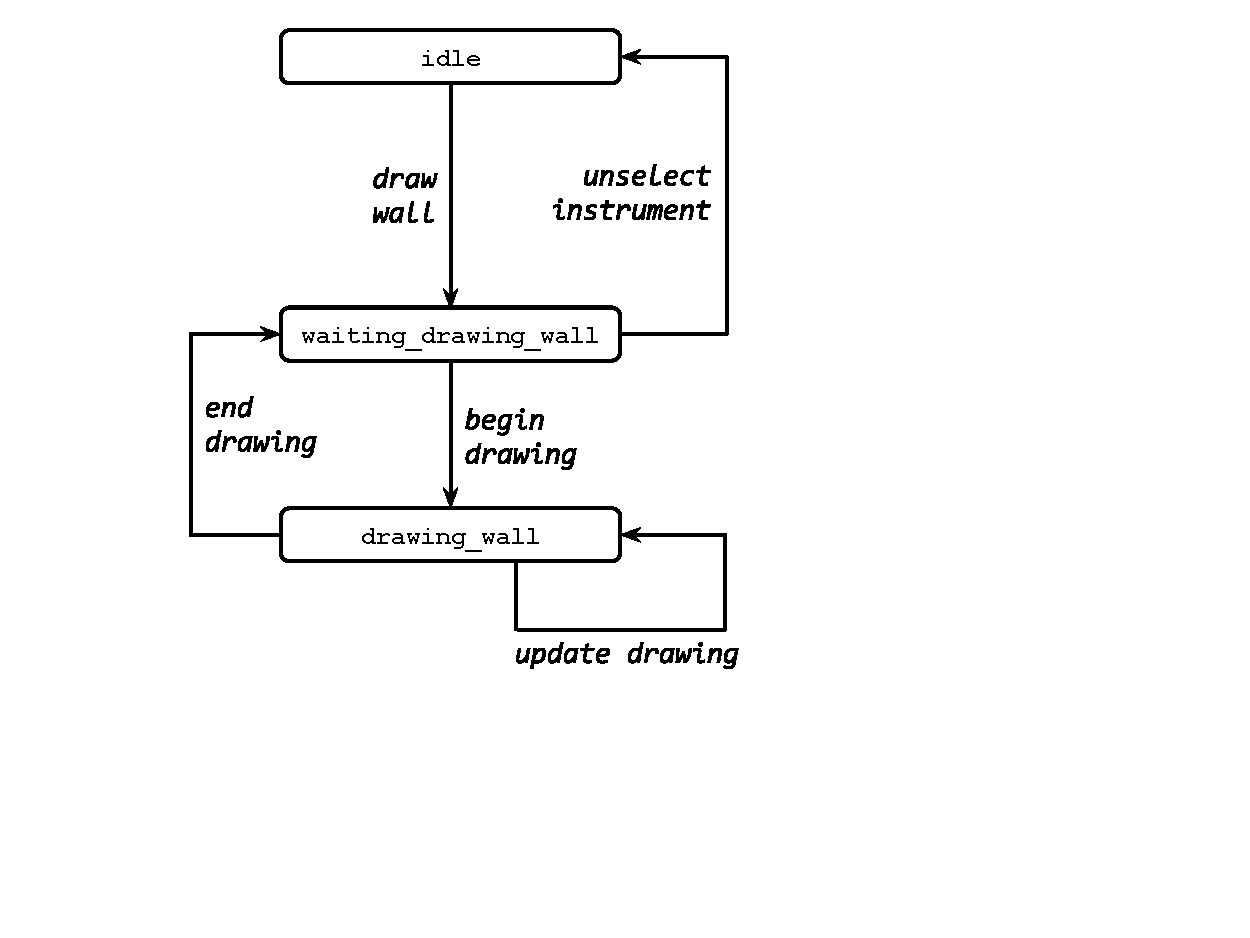
\includegraphics[width=\linewidth]{contents/images/uc_draw_wall}

\caption{Bla bla bla.}
\label{fig_sim}
\end{figure}